
\documentclass[11pt,a4paper]{article}
\usepackage[utf8]{inputenc}
\usepackage[T1]{fontenc}
\usepackage[spanish,es-nodecimaldot]{babel}
\usepackage[a4paper,left=1.7cm,right=1.7cm,top=20mm,bottom=20mm]{geometry}
\usepackage{amsmath,amssymb,amsfonts,mathtools,bm}
\usepackage{braket}
\usepackage{graphicx}
\usepackage{float}
\usepackage{booktabs}
\usepackage{enumitem}
\usepackage{xcolor}
\usepackage{lmodern,microtype}
\usepackage{fancyhdr}
\usepackage{titlesec}
\usepackage[colorlinks=true,linkcolor=black,urlcolor=black,citecolor=black]{hyperref}
\numberwithin{equation}{section}
\renewcommand{\boxed}[1]{#1}
\setlength{\parindent}{0pt}
\setlength{\parskip}{5pt}
\newcommand{\dd}{\,\mathrm d}
\newcommand{\ii}{\mathrm i}
\newcommand{\e}{\mathrm e}
\newcommand{\hb}{\hbar}
\newcommand{\R}{\mathbb R}
\newcommand{\C}{\mathbb C}
\newcommand{\id}{\mathbb I}

\pagestyle{fancy}
\setlength{\headheight}{14pt}
\fancyhf{}
\fancyhead[L]{\textit{Tarea 10}}
\fancyhead[R]{Mecánica Cuántica I}
\begin{document}
\begin{titlepage}
\centering
\vspace*{1.8cm}

\includegraphics[width=.22\textwidth]{UdeC_escudo.png}
\vspace{1.1cm}

{\Huge\bfseries Tarea 10\par}
\vspace{.4cm}
{\Huge\bfseries Mecánica Cuántica I\par}
\vspace{1.5cm}
{\Large José Ignacio Rosas Sepúlveda\par}
\vspace{.8cm}
{\Large Solución\par}
\vfill
\thispagestyle{empty}
\end{titlepage}
\tableofcontents
\newpage
\section*{Enunciado}
\addcontentsline{toc}{section}{Enunciado}
\begin{enumerate}[label=\arabic*.-]
\item Demuestre que dos observables $A$ y $B$ conmutan si y sólo si $A$ y $B$ tienen los mismos estados propios. Use las descomposiciones espectrales
\begin{equation}
A=\sum_n a_n\ket{a_n}\bra{a_n},\qquad
B=\sum_m b_m\ket{b_m}\bra{b_m},
\end{equation}
con bases ortonormales. Calcule el operador conmutador entre ellos y extraiga sus conclusiones.
\item Los estados propios y valores propios de energía de una partícula en una caja de ancho $a$ son
\begin{equation}
\ket{\phi_n}=\sqrt{\frac2a}\int_0^a\sin\left(\frac{n\pi x}{a}\right)\ket x\,\dd x,
\qquad E_n=\frac{\hbar^2\pi^2}{2ma^2}n^2.
\end{equation}
Inicialmente
\begin{equation}
\ket{\psi(0)}=N\int_0^{a/4}x^2(4x-a)^2\ket x\,\dd x,
\end{equation}
donde $N$ es real y positivo.
\begin{enumerate}[label=\alph*)]
\item Demuestre que $N=96\sqrt{70/a^9}$.
\item Encuentre $\psi(x,0)=\braket{x|\psi(0)}$.
\item Encuentre $\psi(p,0)=\braket{p|\psi(0)}$.
\item Encuentre $c_n=\braket{\phi_n|\psi(0)}$.
\item Grafique $a|\psi(x,0)|^2$ como función de $x/a$.
\item Grafique $(\hbar/a)|\psi(p,0)|^2$ como función de $p/(\hbar/a)$.
\item Grafique $|c_n|^2$ como función de $n$.
\end{enumerate}
\end{enumerate}
En lo posible, comente sus resultados.


\section{Problema 1}
Siguiendo la descomposición espectral usada en la clase, escribimos los observables en bases ortonormales de estados propios. Si dos observables hermíticos $A$ y $B$ poseen una base ortonormal completa común $\{\ket n\}$,
\begin{equation}
A=\sum_na_n\ket n\bra n,\qquad B=\sum_nb_n\ket n\bra n,
\end{equation}
Entonces
\begin{align}
AB&=\sum_{n,m}a_nb_m|n\rangle\langle n|m\rangle\langle m|\\
&=\sum_n a_nb_n|n\rangle\langle n|,
\end{align}
y de la misma forma $BA$ produce la misma suma. Por tanto
\begin{equation}
AB=\sum_na_nb_n\ket n\bra n=BA.
\end{equation}
Recíprocamente, si $[A,B]=0$ y $A|a\rangle=a|a\rangle$, entonces
\begin{equation}
A(B|a\rangle)=B(A|a\rangle)=a(B|a\rangle).
\end{equation}
Así, $B|a\rangle$ permanece dentro del subespacio propio de $A$ con valor propio $a$. En un subespacio degenerado se diagonaliza allí la restricción hermítica de $B$. De esta manera ambos operadores admiten una base ortonormal completa común. Como $B$ es hermítico, puede diagonalizarse dentro de cada subespacio degenerado de $A$. De este modo existe una base ortonormal completa que diagonaliza simultáneamente a ambos operadores.

\paragraph{Observación.}
La frase ``tienen los mismos estados propios'' debe entenderse como ``admiten una base completa común de estados propios''. Si $A$ tiene degeneración, no todo vector propio arbitrario de $A$ tiene por qué ser también propio de $B$.


\section{Problema 2}
El desarrollo sigue el mismo procedimiento de cambio de representación de la clase: normalizar el estado en posición y luego proyectarlo sobre las bases $\{|p\rangle\}$ y $\{|\phi_n\rangle\}$.

El estado es
\begin{equation}
\ket{\psi(0)}=N\int_0^{a/4}x^2(4x-a)^2\ket x\dd x.
\end{equation}
Con $y=x/a$,
\begin{equation}
1=N^2a^9\int_0^{1/4}y^4(4y-1)^4\dd y.
\end{equation}
Expandiendo $(4y-1)^4$ e integrando término a término,
\begin{equation}
\int_0^{1/4}y^4(4y-1)^4\,\mathrm dy=\frac{1}{645120}.
\end{equation}
Por tanto $N^2a^9/645120=1$, de donde
\begin{equation}
\boxed{N=96\sqrt{\frac{70}{a^9}}.}
\end{equation}
La función de onda de posición es
\begin{equation}
\boxed{\psi(x,0)=\begin{cases}
96\sqrt{70/a}\,(x/a)^2(4x/a-1)^2,&0\le x\le a/4,\\
0,&\text{fuera de ese intervalo}.
\end{cases}}
\end{equation}

\subsection{Representación de momento}
Definimos $\kappa=pa/\hb$ y
\begin{equation}
F(\kappa)=\int_0^{1/4}y^2(4y-1)^2\e^{-\ii\kappa y}\dd y.
\end{equation}
Para $\kappa\neq0$,
\begin{equation}
F(\kappa)=\frac{2}{\kappa^5}\left[
(-\ii\kappa^2-24\kappa+192\ii)\e^{-\ii\kappa/4}
+(\ii\kappa^2-24\kappa-192\ii)\right],
\end{equation}
y por continuidad $F(0)=1/1920$. Por tanto,
\begin{equation}
\boxed{\psi(p,0)=96\sqrt{70}\sqrt{\frac{a}{2\pi\hb}}\,F(pa/\hb).}
\end{equation}

\subsection{Componentes de energía}
Los estados de la caja son $\phi_n=\sqrt{2/a}\sin(n\pi x/a)$. Así,
\begin{equation}
c_n=96\sqrt{140}\int_0^{1/4}y^2(4y-1)^2\sin(n\pi y)\dd y,
\end{equation}
lo que se reduce a
\begin{equation}
\boxed{c_n=\frac{384\sqrt{35}}{\pi^5n^5}
\left[\pi^2n^2\left(\cos\frac{n\pi}{4}-1\right)
-24\pi n\sin\frac{n\pi}{4}-192\cos\frac{n\pi}{4}+192\right].}
\end{equation}
La distribución de energía es $P(E_n)=|c_n|^2$.

\begin{figure}[H]\centering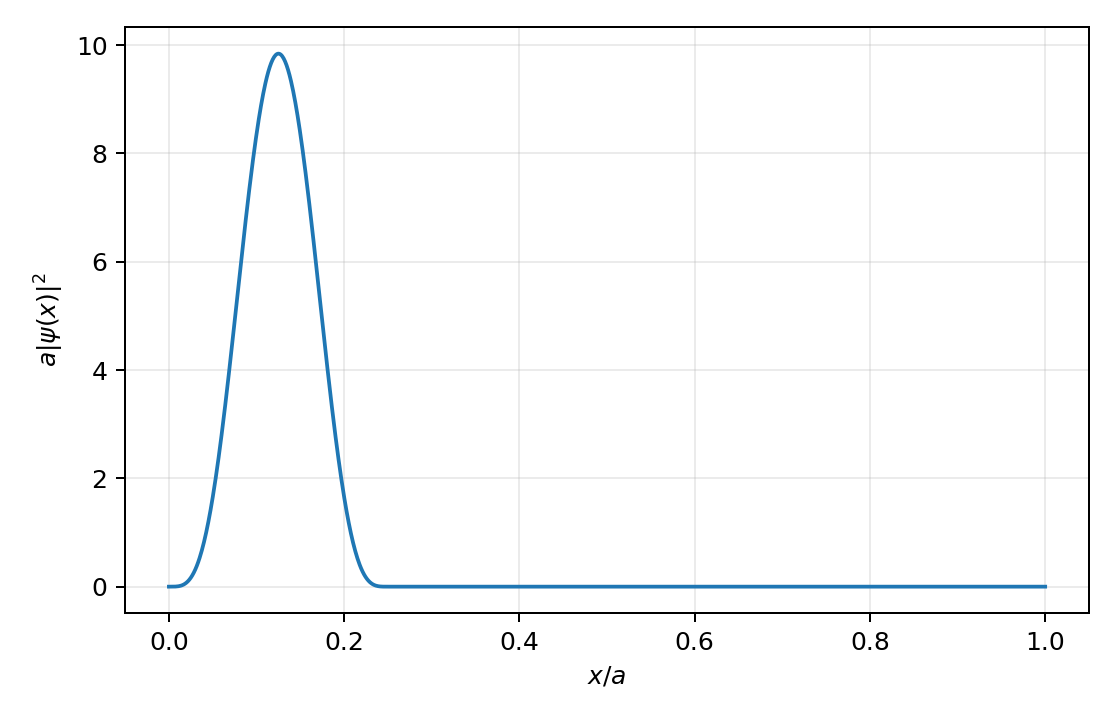
\includegraphics[width=.68\textwidth]{figures/densidad_posicion.png}\caption{Densidad de posición escalada.}\end{figure}
\begin{figure}[H]\centering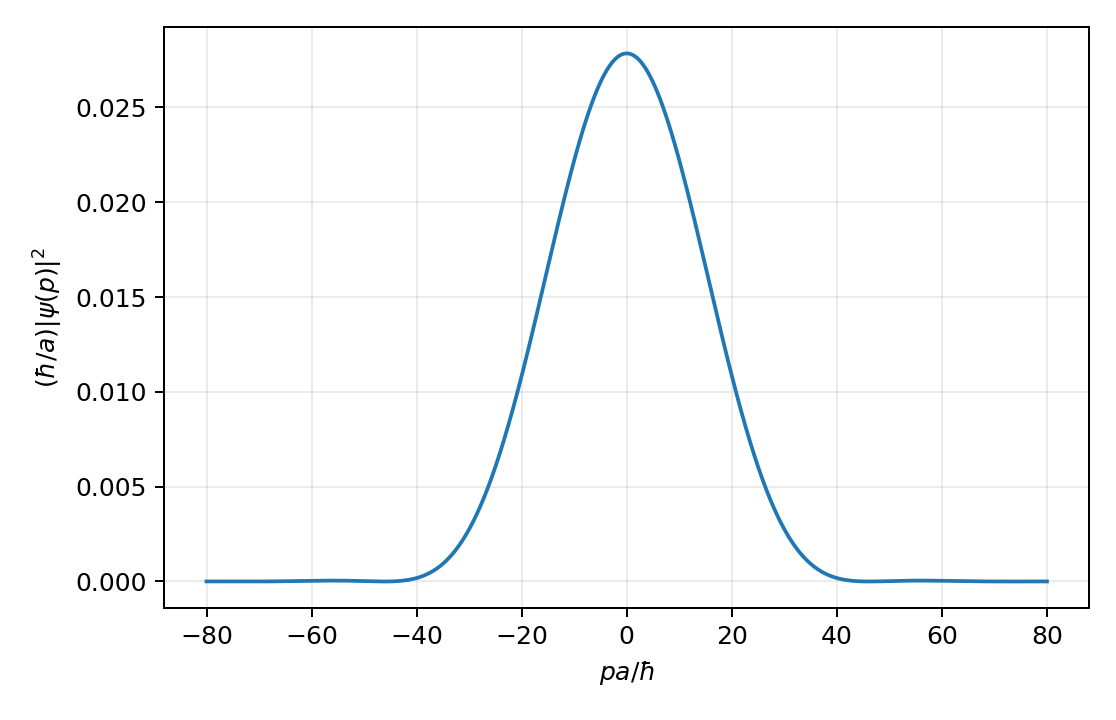
\includegraphics[width=.68\textwidth]{figures/densidad_momento.png}\caption{Densidad de momento escalada.}\end{figure}
\begin{figure}[H]\centering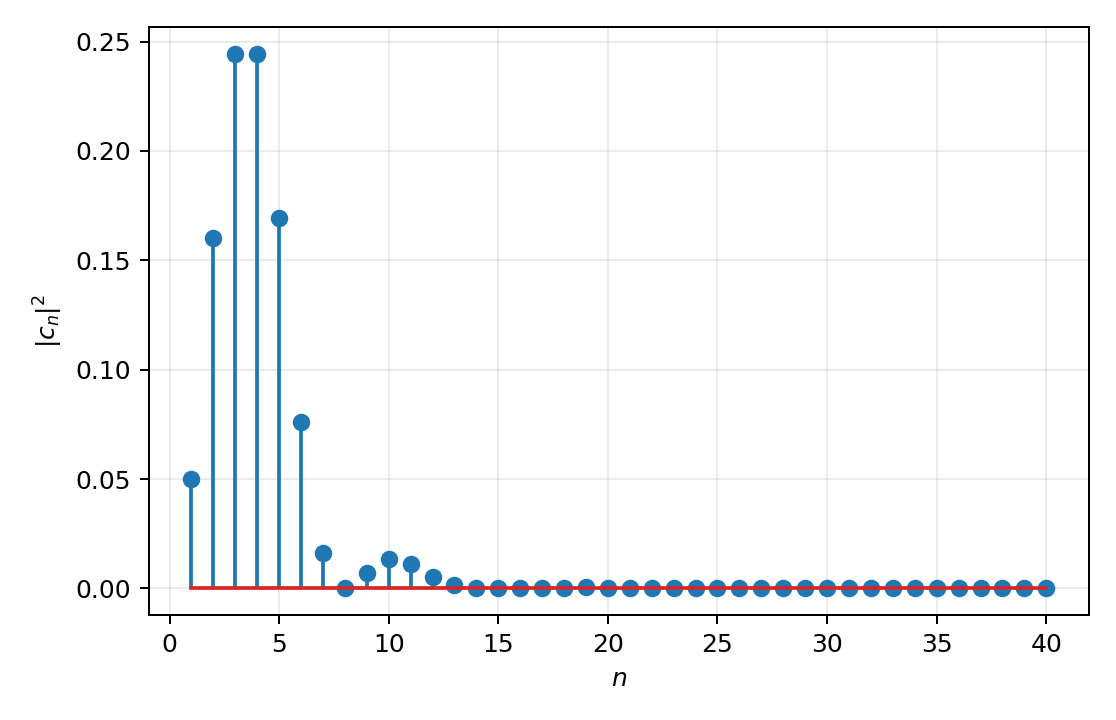
\includegraphics[width=.68\textwidth]{figures/prob_energia.png}\caption{Primeros términos de la distribución de energía.}\end{figure}

\paragraph{Comentario.}
El estado está espacialmente concentrado en $0\le x\le a/4$, por lo que su distribución de momento es ancha. Del mismo modo, la descomposición en energía requiere muchos estados estacionarios: la localización espacial y la presencia de bordes internos agudos demandan componentes de alta frecuencia espacial.



\end{document}
